%!TEX root = ./options_notes.tex

\documentclass[12pt, a4paper]{article}
\usepackage{geometry}
\usepackage{mathtools}
\usepackage{enumitem}
\usepackage{fullpage}
\usepackage{graphicx}
\usepackage{amsmath}
\usepackage{hyperref}


\newcommand{\code}[1]{\texttt{#1}}

\newcommand\Perm[2][^n]{\prescript{#1\mkern-2.5mu}{}P_{#2}}
\newcommand\Comb[2][^n]{\prescript{#1\mkern-0.5mu}{}C_{#2}}

\setlength{\parindent}{0pt} % Set paragraph indent to 0 spaces

\graphicspath{./}

\geometry{a4paper, margin=0.7in}

\begin{document}
\medskip

\section*{Overview on Options}
\subsection*{Features}
\begin{itemize}
    \item Its value depends on the price/price changes of the underlying asset
    \item Has 2 types of options, Call/Puts, Right to Buy/Right to Sell
    \item Exercise/Strike price is the agreed upon price to trade the underlying security
    \item Expiry, is the last date the option holder can exercise the rights of the option
    \item Exercise Style, American/European. American style options can be exercised at any time
          European style options can only be exercised on the expiry date
    \item Premium = Market Price of the Option paid by option buyer to option seller
\end{itemize}

\pagebreak
\section*{Options' Premium Mechanics}
$$ Options'\: Premium/Value = Intrinsic\: Value + Time\: Value $$

The option exercise price, the current share price and the days to expiry are known precisely (Perfect Information).
Volatility of the underlying shares, interest rates and dividends must be estimated  (Imperfect Information).

See: \href{https://www.asxoptions.com/price-calculator/}{ASX Theoretical Price Calculator}

\subsection*{Time Value}
Time Value of an option decreases as the share option moves further away from the strike price,
whether in the money or out of the money. Time value is maximised when an option's premium is
at the money.

As time passes, an option's time value decreases exponentially in a process known as 'time decay'.

Cum-dividend, ex-dividend dates should/do not affect the time value of the option.

\subsection*{Volatility}
The more volatile the stock, the higher the option's premium, all else being equal.

2/3 chance price range will be within one standard deviation of current share price

19/20 change price range will be within 2 standard deviations of current share price

\subsubsection*{Historical Volatility (Perfect Information)}
Trader assumes stock price will behave in the future as it has done in the past

\subsubsection*{Implied Volatility (Imperfect Information)}
Volatility assumption behind the current market price of the option

\subsection*{Interest Rates}
The higher the interest rates, the greater the funding benefit. Thus liquidity in times of
high interest rates allows option holders to invest liquid funds and earn interest.

High interest rates \(\rightarrow\) greater cost of funding \(\rightarrow\) less prepared to pay for puts because you withold
receipt of funds for shares that you own.

Increases in interest rates lead to higher call premiums and lower put premiums.

\subsection*{Delta (Options)}
Delta is the amount an option price is expected to move based on a \$1 change in the underlying stock.\\

The delta of a call option is between zero and 1 (or it may be expressed as a percentage) while the delta of a puts option is between zero and -1 (or it may be expressed as a percentage).
\begin{itemize}
    \item An at-the-money call usually has a delta of around 0.5.
    \item The further out of the money an option is, the closer the delta is to zero.
    \item The deeper in the money an option is, the closer the delta is to 1.
\end{itemize}

\pagebreak
\section*{Options Trading Strategy}

If a trader thinks options are undervalued, strategies involving bought options may be more attractive.
If the trader judges that options are overvalued, they may prefer strategies involving written options.

\begin{center}
    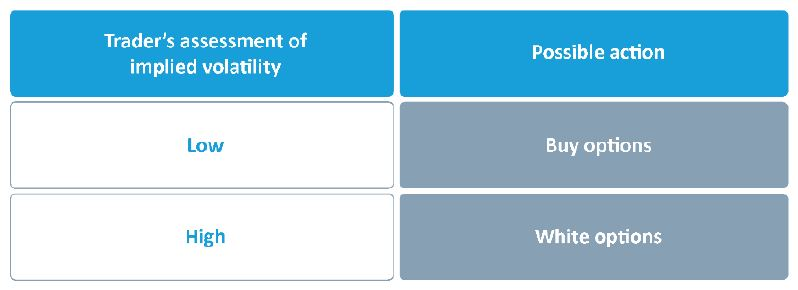
\includegraphics[width=0.5\textwidth]{options_trading_strategy.JPG}
\end{center}

\subsection*{Takers and Writers}
\begin{itemize}
    \item The \textbf{option taker} tries to buy options for as little as possible and then see the option rise in value, at which point they
          sell.
    \item The \textbf{option writer} tries to sell options for as much as possible, and then see the option fall in value, at which point they
          close out the position, or the option expires worthless.
\end{itemize}

In both scenarios, the trader wants to pay as little premium when buying, and receive as much premium when selling,
as possible.

\begin{center}
    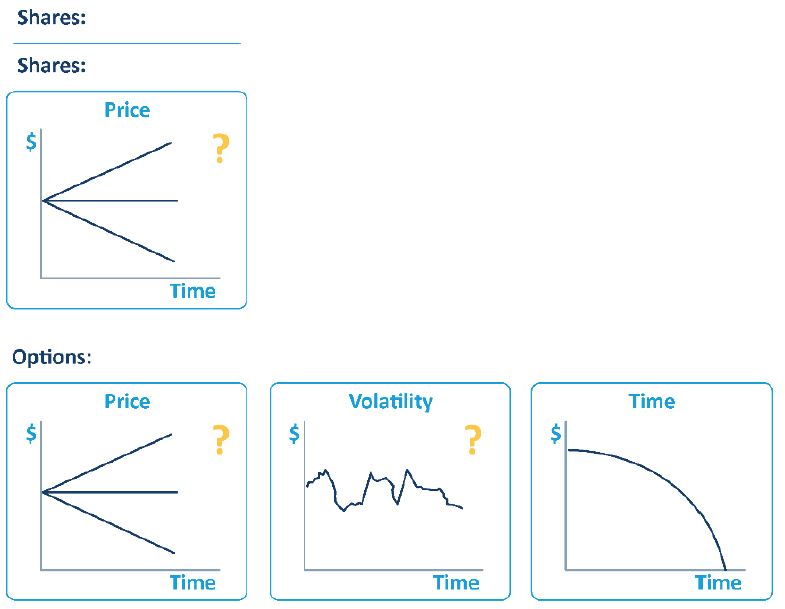
\includegraphics[width=0.6\textwidth]{options_strategy_graph}
\end{center}

\begin{center}
    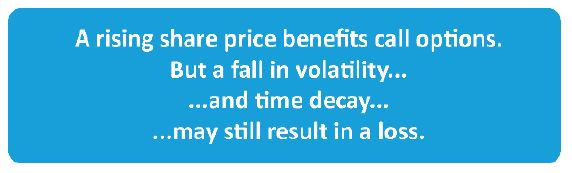
\includegraphics[width=0.5\textwidth]{trading_strategy_note}
\end{center}

\begin{center}
    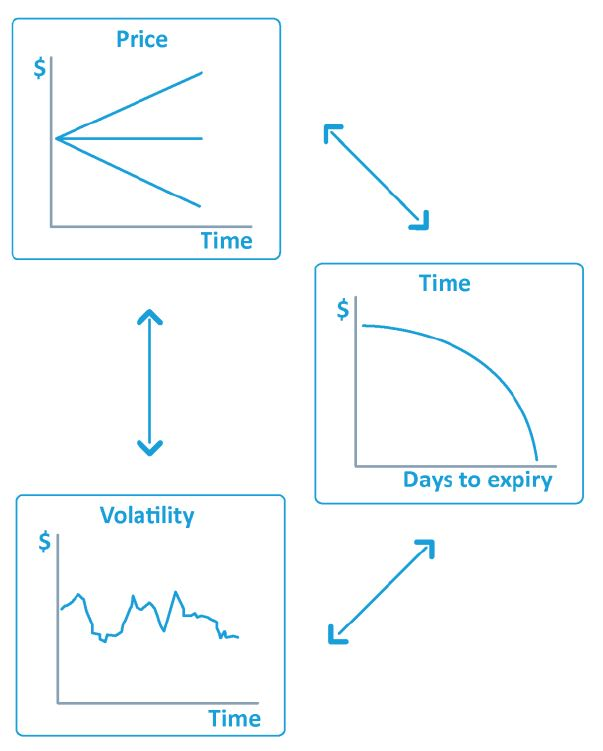
\includegraphics[width=0.5\textwidth]{options_strategy_relations}
\end{center}

\subsection*{Estimating Share Price Movements}
Most investors use either fundamental analysis, or technical analysis, or an approach that combines the two to estimate price movements.
\begin{itemize}
    \item \textbf{Fundamental analysis} involves the study of financial and other information about the company and the industry
          sector, as well as consideration of broad economic data.
    \item \textbf{Technical analysis} is the study of a stock's previous price behaviour, in the belief that patterns repeat themselves and
          can be used to predict future price movements.
\end{itemize}

\subsection*{Volatility}
Volatility affects the value of options.
The higher the volatility, the higher the option premiums as volatiltiy is direction-agnostic and option buyers expect changes in price.\\

When appraising the premium of an option, it is important to form a view on the stock volatility for the life of the option.

\pagebreak
\subsection*{Market Makers}
\subsubsection*{Market Maker benchmarks}
\begin{itemize}
    \item Minimum of 50\% of the required Continuous Quoting benchmark.
    \item Minimum of 50\% of the required Quote Request Quoting benchmark.
    \item A combined minimum average of 70\% on Continuous Quoting and Quote Request Quoting.
\end{itemize}


\end{document}